\documentclass[10pt,a4paper,headsepline,smallheadings]{scrartcl}
\usepackage[utf8]{inputenc}
\usepackage[T1]{fontenc}
\usepackage[ngerman]{babel}
\usepackage{amsmath}
\usepackage{amsthm}
\usepackage{amssymb}
\usepackage{amsfonts}
\usepackage[scaled]{helvet}
\usepackage{amssymb}
\usepackage{multirow}
\usepackage{textcomp}
\usepackage{graphicx}
\usepackage{paralist}
\usepackage{textcomp}
\usepackage{pdflscape} 
\usepackage{marvosym}
\usepackage{float}
\usepackage{siunitx}
\usepackage[siunitx,european,cuteinductors,smartlabels]{circuitikz}
\usepackage{fancyhdr}
\usepackage{pgfplots}
\usepackage{sansmath}
\usepackage{lscape}
\usepackage{multicol}

\usetikzlibrary{calc}


\theoremstyle{definition}
\newtheorem{aufgabe}{Aufgabe}


\renewcommand*\familydefault{\sfdefault}
\renewcommand{\arraystretch}{1.1}


\KOMAoptions{parskip=half,DIV=15,fontsize=11pt}
\unitlength1cm
\titlehead{

\begin{center}\begin{tabular}{p{10cm}p{6.8cm}}
\textbf{FH Aachen} & \textbf{FB Maschinenbau und Mechatronik}\\[0.5cm]
\textbf{Modul 86512} &  Prof. Dr. Raphael Pfaff\\
Herstellung und Vermarktung& Sommersemester 2015\\
\end{tabular}

\end{center}
\begin{picture}(0,0)(0,0)\put(17,-23){
\includegraphics[height=5cm]{fh_logo}}\end{picture}
}
\newif\ifuelsg %als slides
%\uelsgtrue
\uelsgfalse
\newif\ifnotuelsg
\ifuelsg\notuelsgfalse\else\notuelsgtrue\fi
\graphicspath{
{../Bilder/Uebungen/}
{../Bilder/Wirkungsplan/}
}

%\titlehead{83105 \hfill Mess-Steuerungs- und Regelungstechnik \hfill Prof. Manfred Enning}
\title{Herstellung und Vermarktung von Schienenfahrzeugen  -- \"Ubung 1}
\date{}
\makeatletter
\let\Title\@title
\let\Author\@author
\makeatother
\pagestyle{fancy}
\fancyhead[LE, LO]{Prof. Dr. Raphael Pfaff}
\fancyhead[RE, RO]{\Title}

\begin{document}
\thispagestyle{empty}
\maketitle
\vspace{-2cm}
% \hyphenation{Abwei-chungen}

\section*{Projektdokumentation, -planung und -kalkulation}
\begin{minipage}[b]{0.7\textwidth}
Das Labor f\"ur Schienenfahrzeugtechnik der Fachhochschule Aachen m\"ochte einen Sch\"utteltisch zur Durchf\"uhrung von Pr\"ufungen im Bereich Schwingen und Schocken gem\"a{\ss} IEC 61373 anschaffen.

Ziel der Anschaffung ist die Durchf\"uhrung von R\"uttel- und Sch\"utteltests an Schienenfahrzeugkomponenten zur Montage im Wagenkasten. Das Maximalgewicht der Pr\"uflinge betr\"agt 10 kg.

Das Projektbudget betr\"agt 75 kEUR, der Sch\"utteltisch soll zum Sommersemester 2016 betriebsbereit sein.
\end{minipage}
\begin{minipage}[b]{0.3\textwidth}
\begin{center}
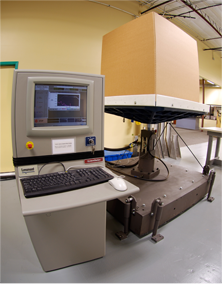
\includegraphics[width=.6\linewidth]{Tester}
\end{center}
\end{minipage}
\vspace{.5cm}

\begin{aufgabe}[Projektdokumentation. Gruppenarbeit 2-3] 
F\"ullen Sie das beiliegende Formular ``Projektauftrag'' aus.
\end{aufgabe}

\begin{aufgabe}[Projektplanung. Gruppenarbeit 2-3] 
Erstellen Sie eine WBS-Analyse zur Feststellung der notwendigen Projektschritte. Sch\"atzen Sie jeweils den erwarteten Aufwand ab. 
\end{aufgabe}

\begin{aufgabe}[Projektplanung. Gruppenarbeit 2-3] 
Stellen Sie die Abh\"angigkeit der Aufgaben in einer Design Structure Matrix dar. Finden Sie Cluster und stellen Sie diese als Subprojekte dar.
\end{aufgabe}

\begin{aufgabe}[Projektplanung. Gruppenarbeit 2-3] 
Stellen Sie den zeitlichen Verlauf im Gantt-Diagramm dar (Vorlage auf n\"achster Seite). Bilden Sie Gruppen und markieren Sie den kritischen Pfad des Projekts.
\end{aufgabe}

\begin{aufgabe}[Projektplanung. Gruppenarbeit 2-3] 
Identifizieren Sie Projektrisiken und definieren Sie Gegenma{\ss}nahmen.
\end{aufgabe}

\begin{aufgabe}[Projektkalkulation. Gruppenarbeit 2-3] 
Kalkulieren Sie auf der Grundlage der WBS die NRC des Projekts auf Seiten der Fachhochschule und bestimmen Sie einen Angebotspreis bei einem Stundensatz von 80 EUR, einem Overhead von 10\% auf Material und Lohnkosten sowie einer kalkulatorischen Marge von 5\%. Bei welcher Verschlechterung der Projektkosten erwirtschaften Sie nur noch den Deckungsbeitrag?
\end{aufgabe}


\begin{landscape}
\begin{center}
\begin{tabular}{l|c|c|c|c|c|c|c|c|c|c|c|c|c}
Action Item \hspace{1cm} & Pre & Dur & May 15 & Jun 15 & Jul 15 & Aug 15 & Sep 15 & Oct 15 & Nov 15 & Dec 15 & Jan 16 & Feb 16 & Mar 16\\ \hline 
& & & & & & & & & & & & &\\[10pt] \hline 
& & & & & & & & & & & & &\\[10pt] \hline 
& & & & & & & & & & & & &\\[10pt] \hline 
& & & & & & & & & & & & &\\[10pt] \hline 
& & & & & & & & & & & & &\\[10pt] \hline 
& & & & & & & & & & & & &\\[10pt] \hline 
& & & & & & & & & & & & &\\[10pt] \hline 
& & & & & & & & & & & & &\\[10pt] \hline 
& & & & & & & & & & & & &\\[10pt] \hline 
& & & & & & & & & & & & &\\[10pt] \hline 
& & & & & & & & & & & & &\\[10pt] \hline 
& & & & & & & & & & & & &\\[10pt] \hline 
& & & & & & & & & & & & &\\[10pt] \hline 
& & & & & & & & & & & & &\\[10pt] \hline 
& & & & & & & & & & & & &\\[10pt] \hline 
& & & & & & & & & & & & &\\[10pt] \hline 
& & & & & & & & & & & & &\\[10pt] \hline 
& & & & & & & & & & & & &\\[10pt] 
\end{tabular}
\end{center}
\end{landscape}
\end{document}